%%
%% This is file `styleguide.tex',
%% generated with the docstrip utility.
%%
%% The original source files were:
%%
%% 6033dp1.dtx  (with options: `styleguide')
%% 
%% Copyright (C) 2009 by the Writing Across the Curriculum staff
%% 
%% All rights reserved.
%% 
\documentclass[strict]{6033dp1}

\title{Style Specification: A Guide to Formatting \\
  Conventions for the DP1 Report}
\author{Writing Across the Curriculum Staff}
\date{March 13, 2009}

\usepackage{graphicx}

\begin{document}
\maketitle

\section{Introduction and Overview}
Technical documents are judged by how completely, clearly, and quickly
they deliver information to a reader.  Skillful use of paragraphing,
sentence structure, and the proper use and definition of technical
terminology will help you create an informative document.  Careful
attention to the formatting of the report will improve its readability
and make information easier to find.

Most organizations that produce professional documents have a style
specification, style sheet, or other document that determines the
overall look of reports and other written material.  Although specific
conventions vary, guidelines help to ensure consistent format within a
particular community of writers.  The guidelines we use are based on
The Mayfield Handbook of Technical and Scientific Writing

\url{https://web.mit.edu/course/21/21.guide/www/home.htm}

For a complete discussion of any topic mentioned in this document,
follow the link to refer to the Mayfield Handbook.

\subsection{Global Document Format}
The following conventions allow you to give your report a professional
look and make information easy for the reader to find.  Writers can
achieve a clear, legible page layout using most generally available
text editing, word processing, or document production programs.

\begin{itemize}
\item Text should be single-spaced, left-justified (ragged right
  margin).  Leave one extra line space between paragraphs.
\item Use a single-column layout.
\item Font should be standard, 11- or 12-point.  You may use a second
  typeface or type style for headings, captions, and other special
  text.  Use these special effects sparingly.
\end{itemize}

\subsubsection{Headings}
Headings should stand out clearly from the running text of your
report.  \uline{Levels} of headings should be easy to identify; the
reader should easily distinguish high-level information from details
and examples.

You may indicate levels of headings through the use of type size and
style.  For a short document such as the DP1 report, which is limited
to 2500 words, too many levels of headings can be confusing.  Use just
\uline{three levels}.

Table~\ref{headingstyles} gives examples of the formatting styles for
three levels of section headings.

\begin{table}[!h]
  \caption{Heading Levels and Styles}
  \label{headingstyles}
  \begin{fulltabular}{|X|X|X|}
    \hline
    \thead{Unnumbered Headings} & \thead{Numbered Headings}\\
    \hline
    {\bfseries\Large Main Heading} &%
                         {\bfseries\Large 1.0 Main Heading}\\
    \hline
    {\bfseries\large Second-Level Heading} &%
                 {\bfseries\large 1.1 Second-Level Heading}\\
    \hline
    {\bfseries Third-Level Heading} &%
                      {\bfseries 1.1.1 Third-Level Heading}\\
    \hline
    {\bfseries Another Third-Level Heading} &%
              {\bfseries 1.1.2 Another Third-Level Heading}\\
    \hline
  \end{fulltabular}
\end{table}

For more information on headings, see:\\
\url{https://web.mit.edu/course/21/21.guide/www/headxsh.htm}

\subsection{Paragraphs and Logical Units of Information}
Readers of technical writing tend to skim documents, read them out of
order, and refer to sections that contain information they
particularly need.  Because readers have such a variety of styles of
using a document, they rely on writers to arrange information by topic
and to establish a clear progression of ideas.

If you craft a paragraph's first sentence carefully, that sentence can
establish context for the rest of the information in the paragraph and
announce the structure for presenting that information.  These first
sentences may be referred to as \uline{topic sentences},
contextualizing statements, or point sentences.  Spend extra time on
first sentences, and make sure that paragraphs are unified, focused,
and coherent.

Use \uline{bulleted and numbered lists} sparingly, and do not use them
to substitute for full discussions or explanations.  Lists should be
introduced with a short paragraph that explains and supplies context
for the items in the list.  Make sure that the items in the list
belong together and that they are grammatically parallel.

For example, you might begin each item with a boldface term and one or
more sentences explaining the term.  You might also list a series of
complete sentences or phrases that fit together logically.

For a complete discussion of topic sentences:\\
\url{https://web.mit.edu/course/21/21.guide/www/topic-s.htm}

For more information on the role of paragraphs and sentences, see:\\
\url{https://web.mit.edu/course/21/21.guide/www/paragraf.htm}\\
\url{https://web.mit.edu/course/21/21.guide/www/sentence.htm}

For more information on bulleted lists and other units of information,
see:\\
\url{https://web.mit.edu/course/21/21.guide/www/layout.htm}

\subsection{Guidelines for Graphics}
If you are not accustomed to using graphics to explain concepts, spend
some time looking at the illustrations in your course readings.  Which
graphics are helpful?  Which ones are confusing?  When students
critique the graphics they find in textbooks, manuals, and published
articles, they often complain that these illustrations are cluttered,
inaccurate, or difficult to relate to the concepts explained in
running text.  Give some thought to the specific point being made in
your graphic.  Adding captions, annotations, and figure numbers helps
readers to understand the point being made.

\subsubsection{Integrate graphics and text:}
\begin{itemize}
\item Summarize the intention of the graphic in the body text of your
  report.
\item Place the graphic as close as possible to a description of what
  it illustrates.
\item Use figure numbers and captions so that readers can switch
  attention between text and graphics easily.  Captions do count
  against your word limit, but readers often pay more attention to
  captions than to body text.
\end{itemize}

\begin{itemize}
\item The figure number and title belong under the figure.  You may
  put explanatory text after the figure title.

  For example, see the caption of Figure~\ref{samplefigure}.

  \begin{figure}[!h]
    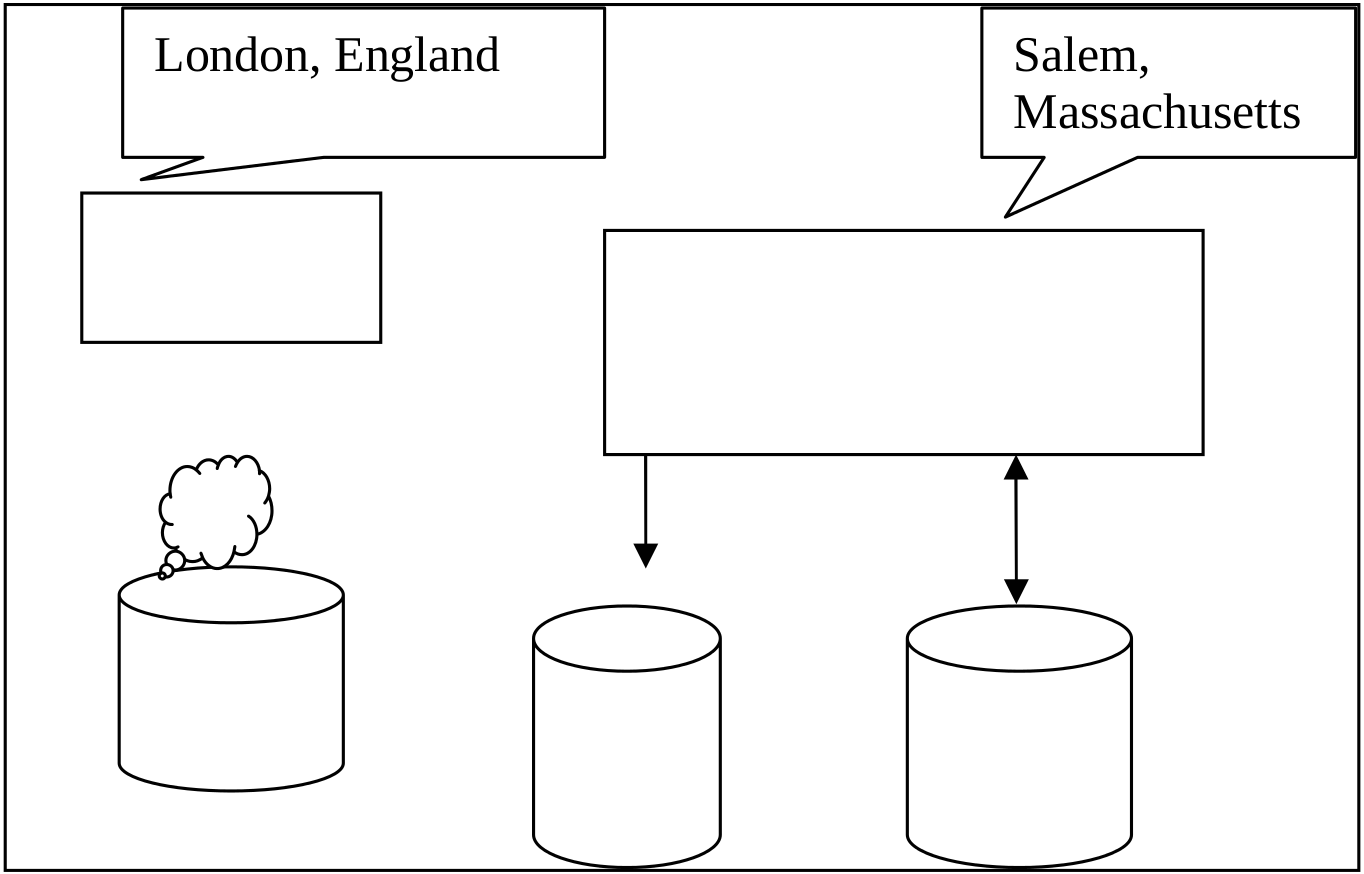
\includegraphics[width=4in]{figure1}
    \caption{A generic illustration.  Note that two unrelated place
      names are featured, and the cylinder on the left appears to be
      sulking.}
    \label{samplefigure}
  \end{figure}

\item In contrast, the table number and title belong \emph{on top of}
  the table, and explanatory text does \emph{not} follow the table
  title.  If necessary, concise explanatory notes may go in small type
  flush under the bottom of the table, as shown in
  Table~\ref{reportedvalues}.

\item Refer to visuals by number only, not position.  For example,
  write ``See Table \ref{reportedvalues}'' not ``See Table
  \ref{reportedvalues} \emph{below}.''

  \begin{table}[!h]
    \caption{Reported values for $a^2 + b^2$}
    \label{reportedvalues}
    \begin{fulltabular}{|X|X|X|}
      \hline
      $a$ & $b$ & $a^2 + b^2$\\
      \hline
      $1$ & $0$ & $1$\\
      \hline
      $2$ & $10$ & $103$\footnotemark[1]\\
      \hline
    \end{fulltabular}

    \small\footnotemark[1] This value is suspect
  \end{table}

\item Use a separate numbering scheme for tables and figures, as
  illustrated by Figure~\ref{samplefigure} and
  Table~\ref{reportedvalues}.  The next figure would be Figure~2, and
  the next table would be Table~III
\end{itemize}

\subsubsection{Emphasize the important detail:}
\begin{itemize}
\item Structure diagrams so important features are emphasized (e.g.,
  by position, labels, bold).  Avoid distracting lines, pictures, or
  special effects.
\item Label the axes of graphs, and specify the units of measurement
  you are using.
\end{itemize}

\subsubsection{Using Pseudocode}
You may use pseudocode examples, if they are kept brief and not used
as a substitute for prose explanations.  Remember that readers want to
see pseudocode as an illustration, but they will not want to decipher
a page of code to understand how your design works.  Pseudocode should
be formatted as a graphic and explained in the text of the report.
For example, the pseudocode in Figure~\ref{rollercoaster} illustrates
the use of 11-point Courier typeface to set it off from the rest of
the report's text, which is 12-point Times Roman.

\begin{figure}[!h]
\begin{lstlisting}
if(height > 60) {
   cout << "You may ride this rollercoaster";
} else {
   cout << Maybe your older sibling will go with you";
}
\end{lstlisting}
  \caption{Pseudocode for rollercoaster riders.}
  \label{rollercoaster}
\end{figure}

The example in Figure~\ref{emperors} shows additional hypothetical
code.  It provides a second illustration of 11-point Courier bold as
contrast with the report's running text:

\begin{figure}[!h]
  \begin{lstlisting}
while(ROME_BURNS) {
   fiddle;
}
  \end{lstlisting}
  \caption{Pseudocode for emperors.}
  \label{emperors}
\end{figure}

For more information on graphics, see:\\
\url{https://web.mit.edu/course/21/21.guide/www/grfxfig.htm}

\subsection{Footnotes}
\uline{Do not use footnotes} in the DP1 Report.  Consider the word
limit, and then weigh the value of any information you plan to include
against the space you have available.  If the information is
important, find a way to incorporate it into the report's running
text.  Bear in mind that any text included in footnotes counts against
the 2500-word limit.

To document your sources, use the IEEE style of in-text citation.  For
more information on IEEE citation, see:

\url{https://web.mit.edu/course/21/21.guide/www/doc-ie3.htm}
\end{document}
\endinput
%%
%% End of file `styleguide.tex'.
